\begin{frame}{Free-Energy Profiles along MFEP's}
\begin{tikzpicture}
\pcuad{\textwidth}{\textheight}
%\showcuad
\path(nw) +(0,0.2) node(cite)[anchor=north west]{\tiny \textcolor{red!80!black}{S. A. Paz, L. Maragliano, and CFA {\em J. Chem. Theory. Comput.} {\bf 14}:2743-2750 (2018)}};
\path(np) +(0,0) node(image)[anchor=north]{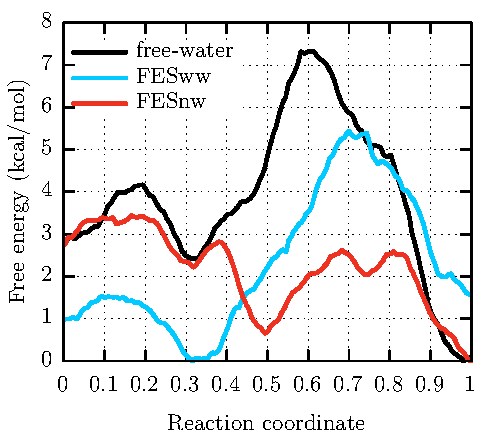
\includegraphics[width=0.67\textwidth]{paths.pdf}};
\path(nw) +(0,-6) node(bullets)[anchor=north west,text width=\textwidth]{\begin{itemize}
\item Energy barriers for unrestricted and ion-tethered water systems are similar; suggests intercalated water is preferred
\item Dry filter shows shallower barriers; dry transport might be faster if water could be actively excluded
\end{itemize}};
\end{tikzpicture}
\end{frame}

